% Options for packages loaded elsewhere
\PassOptionsToPackage{unicode}{hyperref}
\PassOptionsToPackage{hyphens}{url}
%
\documentclass[
]{book}
\usepackage{amsmath,amssymb}
\usepackage{lmodern}
\usepackage{ifxetex,ifluatex}
\ifnum 0\ifxetex 1\fi\ifluatex 1\fi=0 % if pdftex
  \usepackage[T1]{fontenc}
  \usepackage[utf8]{inputenc}
  \usepackage{textcomp} % provide euro and other symbols
\else % if luatex or xetex
  \usepackage{unicode-math}
  \defaultfontfeatures{Scale=MatchLowercase}
  \defaultfontfeatures[\rmfamily]{Ligatures=TeX,Scale=1}
\fi
% Use upquote if available, for straight quotes in verbatim environments
\IfFileExists{upquote.sty}{\usepackage{upquote}}{}
\IfFileExists{microtype.sty}{% use microtype if available
  \usepackage[]{microtype}
  \UseMicrotypeSet[protrusion]{basicmath} % disable protrusion for tt fonts
}{}
\makeatletter
\@ifundefined{KOMAClassName}{% if non-KOMA class
  \IfFileExists{parskip.sty}{%
    \usepackage{parskip}
  }{% else
    \setlength{\parindent}{0pt}
    \setlength{\parskip}{6pt plus 2pt minus 1pt}}
}{% if KOMA class
  \KOMAoptions{parskip=half}}
\makeatother
\usepackage{xcolor}
\IfFileExists{xurl.sty}{\usepackage{xurl}}{} % add URL line breaks if available
\IfFileExists{bookmark.sty}{\usepackage{bookmark}}{\usepackage{hyperref}}
\hypersetup{
  pdftitle={前端学习笔记},
  pdfauthor={刘卢路},
  hidelinks,
  pdfcreator={LaTeX via pandoc}}
\urlstyle{same} % disable monospaced font for URLs
\usepackage{color}
\usepackage{fancyvrb}
\newcommand{\VerbBar}{|}
\newcommand{\VERB}{\Verb[commandchars=\\\{\}]}
\DefineVerbatimEnvironment{Highlighting}{Verbatim}{commandchars=\\\{\}}
% Add ',fontsize=\small' for more characters per line
\usepackage{framed}
\definecolor{shadecolor}{RGB}{248,248,248}
\newenvironment{Shaded}{\begin{snugshade}}{\end{snugshade}}
\newcommand{\AlertTok}[1]{\textcolor[rgb]{0.94,0.16,0.16}{#1}}
\newcommand{\AnnotationTok}[1]{\textcolor[rgb]{0.56,0.35,0.01}{\textbf{\textit{#1}}}}
\newcommand{\AttributeTok}[1]{\textcolor[rgb]{0.77,0.63,0.00}{#1}}
\newcommand{\BaseNTok}[1]{\textcolor[rgb]{0.00,0.00,0.81}{#1}}
\newcommand{\BuiltInTok}[1]{#1}
\newcommand{\CharTok}[1]{\textcolor[rgb]{0.31,0.60,0.02}{#1}}
\newcommand{\CommentTok}[1]{\textcolor[rgb]{0.56,0.35,0.01}{\textit{#1}}}
\newcommand{\CommentVarTok}[1]{\textcolor[rgb]{0.56,0.35,0.01}{\textbf{\textit{#1}}}}
\newcommand{\ConstantTok}[1]{\textcolor[rgb]{0.00,0.00,0.00}{#1}}
\newcommand{\ControlFlowTok}[1]{\textcolor[rgb]{0.13,0.29,0.53}{\textbf{#1}}}
\newcommand{\DataTypeTok}[1]{\textcolor[rgb]{0.13,0.29,0.53}{#1}}
\newcommand{\DecValTok}[1]{\textcolor[rgb]{0.00,0.00,0.81}{#1}}
\newcommand{\DocumentationTok}[1]{\textcolor[rgb]{0.56,0.35,0.01}{\textbf{\textit{#1}}}}
\newcommand{\ErrorTok}[1]{\textcolor[rgb]{0.64,0.00,0.00}{\textbf{#1}}}
\newcommand{\ExtensionTok}[1]{#1}
\newcommand{\FloatTok}[1]{\textcolor[rgb]{0.00,0.00,0.81}{#1}}
\newcommand{\FunctionTok}[1]{\textcolor[rgb]{0.00,0.00,0.00}{#1}}
\newcommand{\ImportTok}[1]{#1}
\newcommand{\InformationTok}[1]{\textcolor[rgb]{0.56,0.35,0.01}{\textbf{\textit{#1}}}}
\newcommand{\KeywordTok}[1]{\textcolor[rgb]{0.13,0.29,0.53}{\textbf{#1}}}
\newcommand{\NormalTok}[1]{#1}
\newcommand{\OperatorTok}[1]{\textcolor[rgb]{0.81,0.36,0.00}{\textbf{#1}}}
\newcommand{\OtherTok}[1]{\textcolor[rgb]{0.56,0.35,0.01}{#1}}
\newcommand{\PreprocessorTok}[1]{\textcolor[rgb]{0.56,0.35,0.01}{\textit{#1}}}
\newcommand{\RegionMarkerTok}[1]{#1}
\newcommand{\SpecialCharTok}[1]{\textcolor[rgb]{0.00,0.00,0.00}{#1}}
\newcommand{\SpecialStringTok}[1]{\textcolor[rgb]{0.31,0.60,0.02}{#1}}
\newcommand{\StringTok}[1]{\textcolor[rgb]{0.31,0.60,0.02}{#1}}
\newcommand{\VariableTok}[1]{\textcolor[rgb]{0.00,0.00,0.00}{#1}}
\newcommand{\VerbatimStringTok}[1]{\textcolor[rgb]{0.31,0.60,0.02}{#1}}
\newcommand{\WarningTok}[1]{\textcolor[rgb]{0.56,0.35,0.01}{\textbf{\textit{#1}}}}
\usepackage{longtable,booktabs,array}
\usepackage{calc} % for calculating minipage widths
% Correct order of tables after \paragraph or \subparagraph
\usepackage{etoolbox}
\makeatletter
\patchcmd\longtable{\par}{\if@noskipsec\mbox{}\fi\par}{}{}
\makeatother
% Allow footnotes in longtable head/foot
\IfFileExists{footnotehyper.sty}{\usepackage{footnotehyper}}{\usepackage{footnote}}
\makesavenoteenv{longtable}
\usepackage{graphicx}
\makeatletter
\def\maxwidth{\ifdim\Gin@nat@width>\linewidth\linewidth\else\Gin@nat@width\fi}
\def\maxheight{\ifdim\Gin@nat@height>\textheight\textheight\else\Gin@nat@height\fi}
\makeatother
% Scale images if necessary, so that they will not overflow the page
% margins by default, and it is still possible to overwrite the defaults
% using explicit options in \includegraphics[width, height, ...]{}
\setkeys{Gin}{width=\maxwidth,height=\maxheight,keepaspectratio}
% Set default figure placement to htbp
\makeatletter
\def\fps@figure{htbp}
\makeatother
\setlength{\emergencystretch}{3em} % prevent overfull lines
\providecommand{\tightlist}{%
  \setlength{\itemsep}{0pt}\setlength{\parskip}{0pt}}
\setcounter{secnumdepth}{5}
\usepackage{ctex}

%\usepackage{xltxtra} % XeLaTeX的一些额外符号
% 设置中文字体
%\setCJKmainfont[BoldFont={黑体},ItalicFont={楷体}]{新宋体}

% 设置边距
\usepackage{geometry}
\geometry{%
  left=2.0cm, right=2.0cm, top=3.5cm, bottom=2.5cm} 

\usepackage{amsthm,mathrsfs}
\usepackage{booktabs}
\usepackage{longtable}
\makeatletter
\def\thm@space@setup{%
  \thm@preskip=8pt plus 2pt minus 4pt
  \thm@postskip=\thm@preskip
}
\makeatother
\ifluatex
  \usepackage{selnolig}  % disable illegal ligatures
\fi
\usepackage[style=apa,]{biblatex}
\addbibresource{mybib.bib}

\title{前端学习笔记}
\author{刘卢路}
\date{2021年9月28日}

\begin{document}
\maketitle

{
\setcounter{tocdepth}{1}
\tableofcontents
}
\hypertarget{ux524dux8a00}{%
\chapter*{前言}\label{ux524dux8a00}}
\addcontentsline{toc}{chapter}{前言}

勤做笔记不仅可以让自己学的扎实,更重要的是可以让自己少走弯路。有人说:``再次翻开笔记是什么感觉'',我的回答是:``怦然心动的感觉''。或许笔记不一定十全十美,但肯定会让你有种心动💖的感觉。

\hypertarget{part-htmlux57faux7840}{%
\part{HTML基础}\label{part-htmlux57faux7840}}

\hypertarget{ux8ba4ux8bc6web}{%
\chapter{认识Web}\label{ux8ba4ux8bc6web}}

本篇文章主要由五个章节构成,从WEB标准到初识HTML,接着学习HTML常用标签,最后学习表格列表和表单。💪💪开始充电之旅啦\textasciitilde\textasciitilde\textasciitilde{}

\hypertarget{ux7f51ux9875}{%
\section{网页}\label{ux7f51ux9875}}

\textbf{网页}是由文字、图像、音频、视频等元素构成。我们通常看到的网页是以.htm或.html后缀结尾的文件,因此将其俗称为HTML文件,它需要通过浏览器来阅读。

\textbf{网站}是网页的集合。

\textbf{HTML}是超文标记语言(Hyper Text Makeup Language),它是一种用来描述网页的一种语言。
HTML不是编程语言,而是一种标记语言(Makeup language),标记语言是一套标签标记(Makeup tag)。
所谓超文本,有两层含义:

\begin{itemize}
\tightlist
\item
  它可以加入图片、声音、动画、多媒体等内容(超越了文本显著)
\item
  它可以从一个文件跳转到另一个文件,与世界各地主机文件连接(炒鸡连接文本)
\end{itemize}

\textbf{网页的形成}
网页是由网页元素组成的,这些元素是利用html标签描述出来,然后通过浏览器解析出来显示给用户。
前端人员开发代码→浏览器显示代码(解析、渲染)→生成Web页面

\hypertarget{ux6d4fux89c8ux5668}{%
\section{浏览器}\label{ux6d4fux89c8ux5668}}

\textbf{浏览器}是显示、运行网页的平台。IE、火狐(Firefox)、谷歌(Chrome)、Safari和欧鹏(Opera)被称为五大浏览器。

\textbf{浏览器内核}排版引擎、解释引擎、渲染引擎。负责读取网页内容,整理讯息,计算网页的显示方式并显示页面。

\begin{table}

\caption{\label{tab:unnamed-chunk-1}浏览器内核}
\centering
\begin{tabular}[t]{lll}
\toprule
浏览器 & 内核 & 备注\\
\midrule
IE & Trident & IE、猎豹安全、360极速浏览器、百度浏览器\\
Firefox & Gecko & 可惜这几年已经没落了,打开速度慢、升级频繁、猪一样的队友flash、神一样的对手chrome。\\
Safari & Webkit & 现在很多人错误地把 webkit 叫做 chrome内核(即使 chrome内核已经是 blink 了)。苹果感觉像被别人抢了媳妇,都哭晕在厕所里面了。\\
Chrome & Chromium/Blink & 在 Chromium 项目中研发 Blink 渲染引擎(即浏览器核心),内置于 Chrome 浏览器之中。Blink 其实是 WebKit 的分支。大部分国产浏览器最新版都采用Blink内核。二次开发\\
Opera & Blink & 现在跟随chrome用blink内核。\\
\bottomrule
\end{tabular}
\end{table}

\hypertarget{webux6807ux51c6}{%
\section{Web标准}\label{webux6807ux51c6}}

Web标准是由W3C组织和其他标准化组织制定的一系列标准的集合。W3C(万维网联盟)是国际最著名的标准化组织。

\hypertarget{ux4e3aux4ec0ux4e48ux9700ux8981webux6807ux51c6}{%
\subsection{为什么需要Web标准}\label{ux4e3aux4ec0ux4e48ux9700ux8981webux6807ux51c6}}

浏览器不同,它们显示页面或者排版就有些许差异。
遵循Web标准除了可以让不同开发人员写出的页面更标准,更统一外,还有以下优点:👇

\begin{itemize}
\tightlist
\item
  易于维护:只需更改CSS文件,就可以改变整站的样式
\item
  页面响应快:HTML文档体积变小,响应时间短
\item
  可访问性:语义化的HTML(结构和表现相分离的HTML)编写的网页文件,更容易被屏幕阅读器识别
\item
  设备兼容性:不同的样式表可以让网页在不同的设备上呈现不同的样式
\item
  搜索引擎:语义化的HTML能更容易被搜索引擎解析,提升排名
\end{itemize}

\hypertarget{webux6807ux51c6ux6784ux6210}{%
\subsection{Web标准构成}\label{webux6807ux51c6ux6784ux6210}}

主要包括结构标准(Structure),表现标准(Presentation)和行为标准(Behavior)。

\begin{itemize}
\tightlist
\item
  结构标准用于对网页元素进行整理和分类,现阶段主要学的是HTML
\item
  表现标准用于设置网页元素的版式、颜色、大小等外观属性,主要指的是CSS
\item
  行为标准用于对网页模型的定义及交互的编写,现阶段主要学的是JavaScript
\end{itemize}

\begin{table}

\caption{\label{tab:unnamed-chunk-2}Web标准}
\centering
\begin{tabular}[t]{ll}
\toprule
标准 & 说明\\
\midrule
结构标准 & 用于对网页元素进行整理和分类,现阶段主要学的是HTML\\
表现标准 & 用于设置网页元素的版式、颜色、大小等外观属性,主要指的是CSS\\
行为标准 & 用于对网页模型的定义及交互的编写,现阶段主要学的是JavaScript\\
\bottomrule
\end{tabular}
\end{table}

Web标准提出的最佳体验方案:\textbf{结构、样式、行为相分离}。简单理解:结构写到HTML文件中、表现写到CSS文件中、行为写到JavaScript中。

\begin{figure}

{\centering 
\includegraphics{fig/1-1} 

}

\caption{Web标准}\label{fig:unnamed-chunk-3}
\end{figure}

\hypertarget{htmlux521dux8bc6}{%
\chapter{HTML初识}\label{htmlux521dux8bc6}}

\hypertarget{ux57faux672cux8bedux6cd5ux89c4ux8303}{%
\section{基本语法规范}\label{ux57faux672cux8bedux6cd5ux89c4ux8303}}

\hypertarget{ux57faux672cux8bedux6cd5ux6982ux8ff0}{%
\subsection{基本语法概述}\label{ux57faux672cux8bedux6cd5ux6982ux8ff0}}

HTML标签是由尖括号包围的关键词,例如\texttt{\textless{}html\textgreater{}}。

HTML标签通常是成对出现的,例如\texttt{\textless{}html\textgreater{}}和\texttt{\textless{}/html\textgreater{}},我们称为双标签。标签对中的第一个标签是开始标签,第二个标签是结束标签。

有些特殊标签必须是单个标签(极少情况),例如\texttt{\textless{}br\ /\textgreater{}},我们称为单标签。

\hypertarget{ux6807ux7b7eux5173ux7cfb}{%
\subsection{标签关系}\label{ux6807ux7b7eux5173ux7cfb}}

双标签关系可以分为两类:包含关系和并列关系。

包含关系,又被称为父子关系。
eg:title标签包含于head标签中。

\begin{Shaded}
\begin{Highlighting}[]
\KeywordTok{\textless{}head\textgreater{}}
    \KeywordTok{\textless{}title\textgreater{}\textless{}/title\textgreater{}}
\KeywordTok{\textless{}/head\textgreater{}}
\end{Highlighting}
\end{Shaded}

并列关系,又被称为兄弟关系。
eg:title标签和head标签并列。

\begin{Shaded}
\begin{Highlighting}[]
\KeywordTok{\textless{}head\textgreater{}\textless{}/head\textgreater{}}
\KeywordTok{\textless{}body\textgreater{}\textless{}/body\textgreater{}}
\end{Highlighting}
\end{Shaded}

\hypertarget{ux57faux672cux7ed3ux6784ux6807ux7b7e}{%
\section{基本结构标签}\label{ux57faux672cux7ed3ux6784ux6807ux7b7e}}

每个网页都会有一个基本的结构标签(也被称为骨架标签),页面内容也是在这些基本标签上书写。HTML页面也称为HTML文档。

\begin{Shaded}
\begin{Highlighting}[]
\KeywordTok{\textless{}html\textgreater{}}
    \KeywordTok{\textless{}head\textgreater{}}     
        \KeywordTok{\textless{}title\textgreater{}}\NormalTok{第一个页面}\KeywordTok{\textless{}/title\textgreater{}} 
    \KeywordTok{\textless{}/head\textgreater{}}
    \KeywordTok{\textless{}body\textgreater{}}
\NormalTok{         键盘敲烂,工资过万}
    \KeywordTok{\textless{}/body\textgreater{}}
\KeywordTok{\textless{}/html\textgreater{}}
\end{Highlighting}
\end{Shaded}

HTML文档的后缀名必须是.htm或.html,浏览器的作用是读取HTML文档,并以网页形式显示他们。此时,用浏览器打开这个网页,我们就可以预览我们写的HTML文件了。

\begin{table}

\caption{\label{tab:unnamed-chunk-4}基本结构标签}
\centering
\begin{tabular}[t]{lll}
\toprule
标题名 & 定义 & 说明\\
\midrule
`<html></html>` & HTML标签 & 页面中最大的标签,我们称为根标签\\
`<head></head>` & 文档头部 & 注意head标签中我们必须要设置的标签是tittle\\
`<title></title>` & 文档标题 & 让页面拥有一个属于自己的网页标题\\
`<body></body>` & 文档主体 & 元素包含文档的所有内容,页面内容基本都是放到body里面\\
\bottomrule
\end{tabular}
\end{table}

\begin{figure}

{\centering 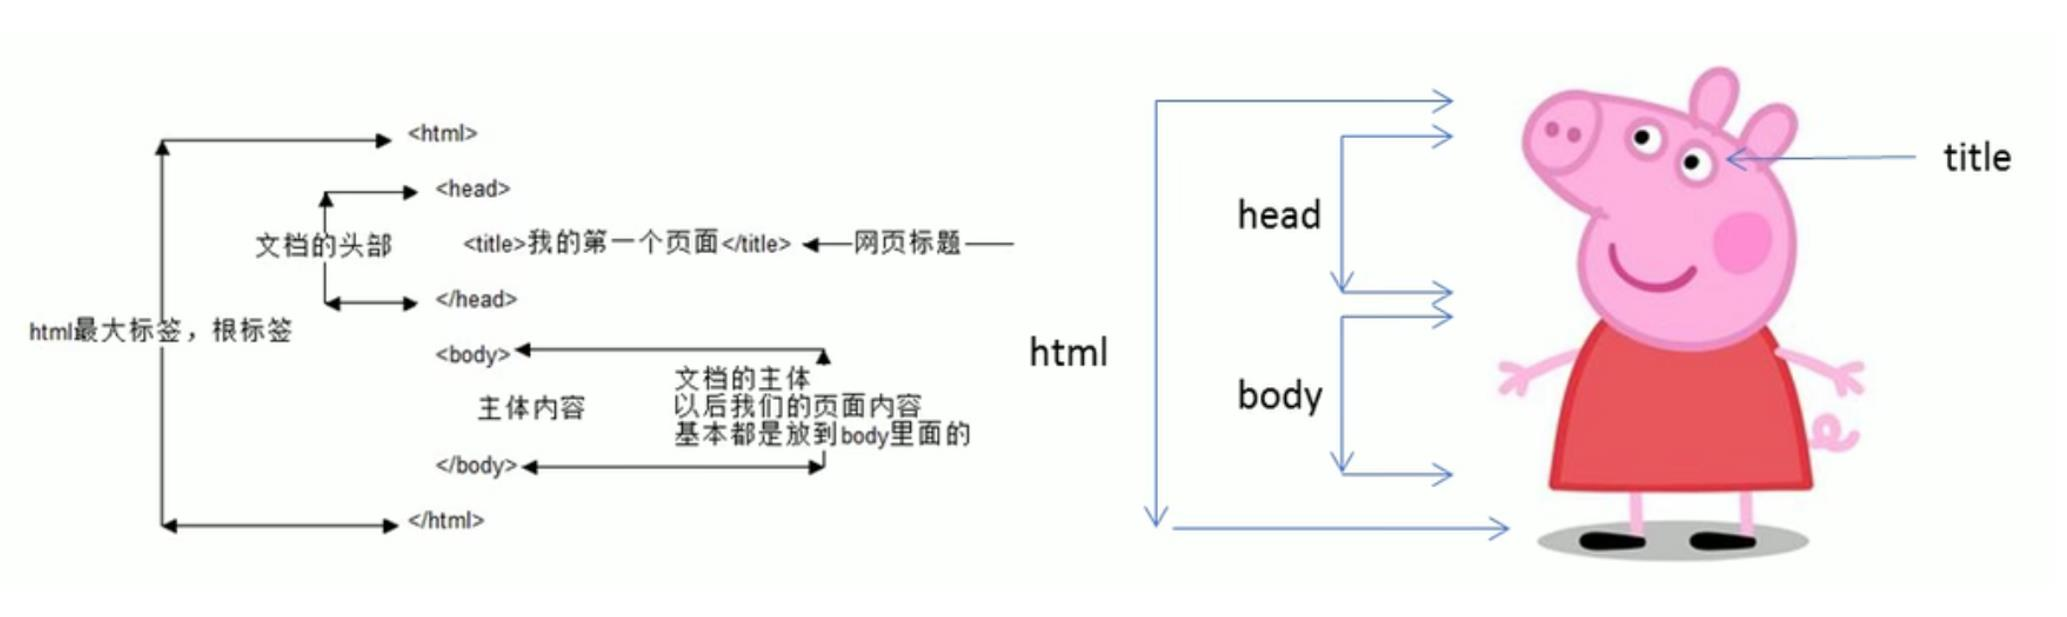
\includegraphics{fig/1-2} 

}

\caption{HTML骨架标签}\label{fig:unnamed-chunk-5}
\end{figure}

\hypertarget{ux7f51ux9875ux5f00ux53d1ux5de5ux5177}{%
\chapter{网页开发工具}\label{ux7f51ux9875ux5f00ux53d1ux5de5ux5177}}

\hypertarget{ux914dux7f6evscode}{%
\section{配置VSCode}\label{ux914dux7f6evscode}}

下载并安装\href{https://code.visualstudio.com/download}{Visual Studio Code软件}

新建文件(快捷键\texttt{Ctrl}+\texttt{N}),然后保存(快捷键\texttt{Ctrl}+\texttt{S})后缀名为.html的文件,在第一行代码中输入\texttt{!},再按\texttt{Tab}键,即可自动生成HTML的骨架文件。安装插件(Open in Browser)后可在浏览器中预览,单击鼠标右键,在弹出窗口中点击\texttt{Open\ in\ Default\ Browser}。\\
接下来介绍一下如何安装插件。

\begin{figure}

{\centering 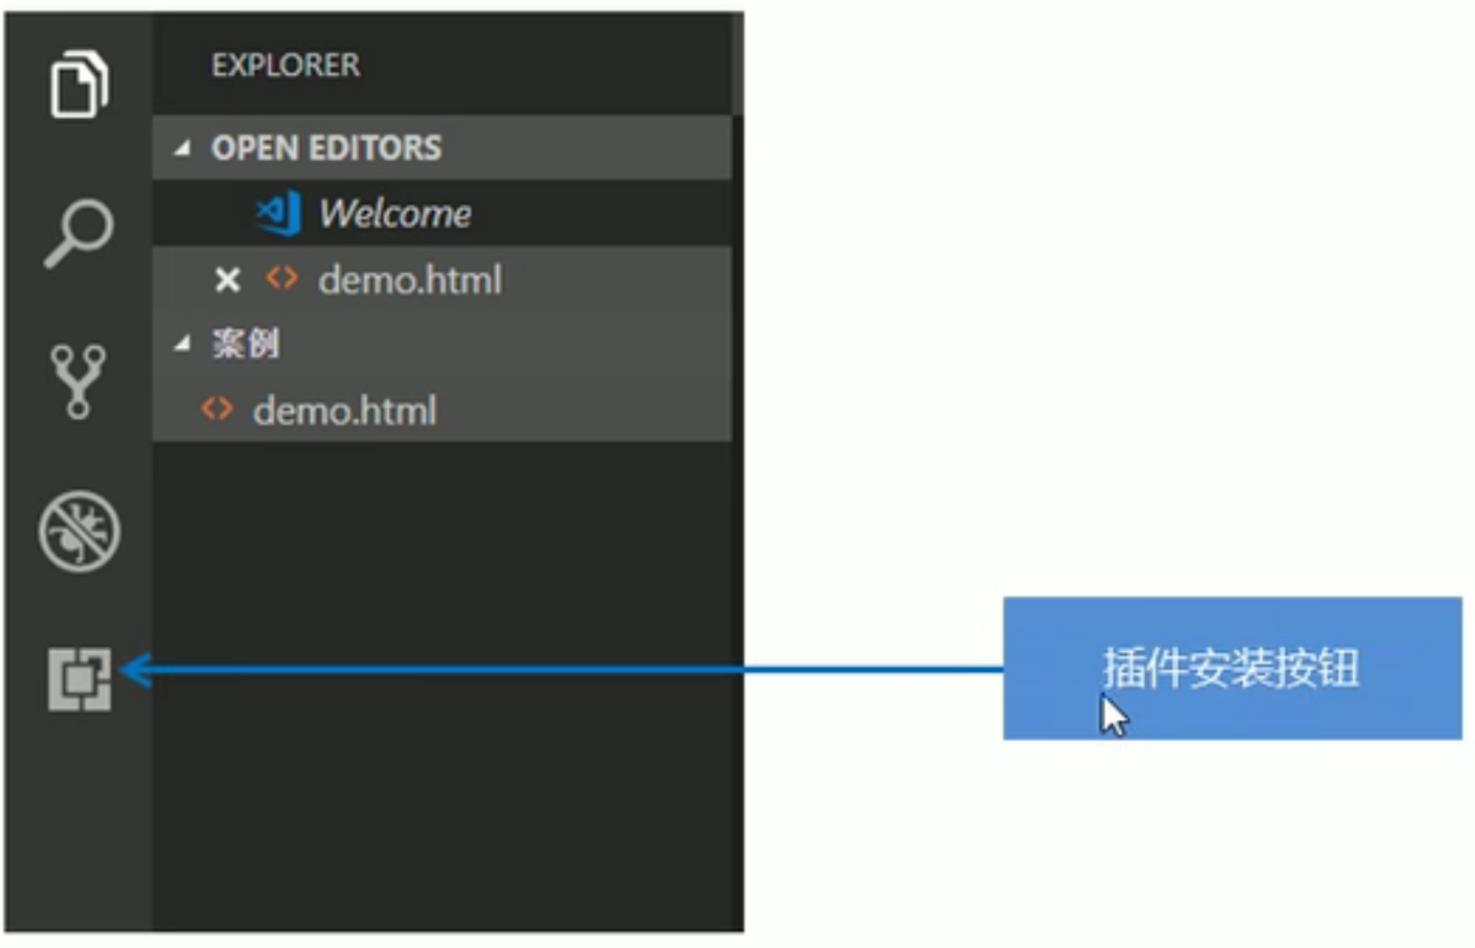
\includegraphics[width=0.5\linewidth]{fig/1-4} 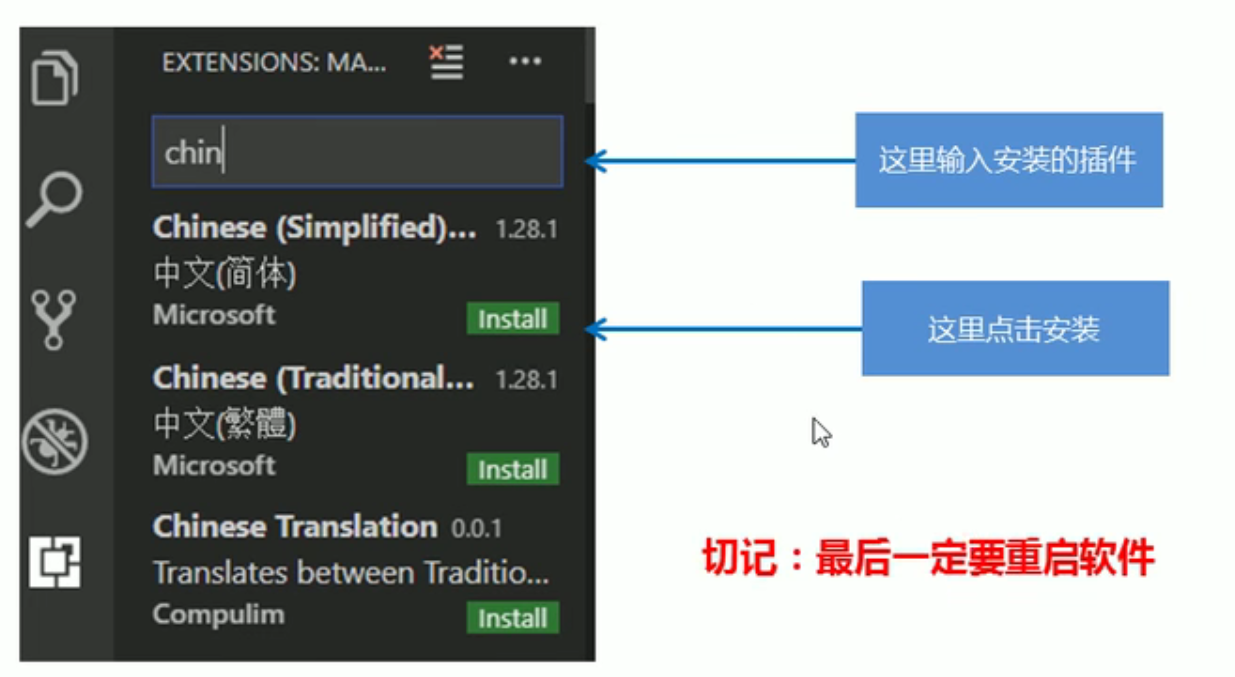
\includegraphics[width=0.5\linewidth]{fig/1-5} 

}

\caption{安装插件}\label{fig:unnamed-chunk-1}
\end{figure}

一些常用的插件:

\begin{table}

\caption{\label{tab:unnamed-chunk-2}基本结构标签}
\centering
\begin{tabular}[t]{ll}
\toprule
插件 & 作用\\
\midrule
Chinese (Simplified) Language Pack of VS Code & 中文(简体)语言包\\
Open in Browser & 右键选择浏览器打开HTML文件\\
JS-CSS-HTML Formatter & 每次保存,都会自动格式化JS CSS和HTML代码\\
Auto Rename Tag & 自动重命名配对的HTML/XML标签\\
CSS peek & 追踪至样式\\
\bottomrule
\end{tabular}
\end{table}

\hypertarget{vscodeux5de5ux5177ux751fux6210ux9aa8ux67b6ux6807ux7b7eux65b0ux589eux4ee3ux7801}{%
\section{VSCode工具生成骨架标签新增代码}\label{vscodeux5de5ux5177ux751fux6210ux9aa8ux67b6ux6807ux7b7eux65b0ux589eux4ee3ux7801}}

下面的代码是VSCode生产的骨架代码

\begin{Shaded}
\begin{Highlighting}[]
\DataTypeTok{\textless{}!DOCTYPE }\NormalTok{html}\DataTypeTok{\textgreater{}}
\KeywordTok{\textless{}html}\OtherTok{ lang=}\StringTok{"en"}\KeywordTok{\textgreater{}}
\KeywordTok{\textless{}head\textgreater{}}
    \KeywordTok{\textless{}meta}\OtherTok{ charset=}\StringTok{"UTF{-}8"}\KeywordTok{\textgreater{}}
    \KeywordTok{\textless{}meta}\OtherTok{ http{-}equiv=}\StringTok{"X{-}UA{-}Compatible"}\OtherTok{ content=}\StringTok{"IE=edge"}\KeywordTok{\textgreater{}}
    \KeywordTok{\textless{}meta}\OtherTok{ name=}\StringTok{"viewport"}\OtherTok{ content=}\StringTok{"width=device{-}width, initial{-}scale=1.0"}\KeywordTok{\textgreater{}}
    \KeywordTok{\textless{}title\textgreater{}}\NormalTok{Document}\KeywordTok{\textless{}/title\textgreater{}}
\KeywordTok{\textless{}/head\textgreater{}}
\KeywordTok{\textless{}body\textgreater{}}
    
\KeywordTok{\textless{}/body\textgreater{}}
\KeywordTok{\textless{}/html\textgreater{}}
\end{Highlighting}
\end{Shaded}

\hypertarget{ux6587ux6863ux7c7bux578bdoctype}{%
\subsection{\texorpdfstring{文档类型\texttt{\textless{}!DOCTYPE\textgreater{}}}{文档类型\textless!DOCTYPE\textgreater{}}}\label{ux6587ux6863ux7c7bux578bdoctype}}

\texttt{\textless{}!DOCTYPE\textgreater{}}是文档类型(Document type)声明,作用是告诉浏览器使用哪种HTML版本来显示网页。

\begin{Shaded}
\begin{Highlighting}[]
\DataTypeTok{\textless{}!DOCTYPE }\NormalTok{html}\DataTypeTok{\textgreater{}}
\end{Highlighting}
\end{Shaded}

这句代码的意思是:当前页面采取的是HTML5版本来显示网页。注意\texttt{\textless{}!DOCTYPE\textgreater{}}声明位于文档中的首行,处于\texttt{\textless{}html\textgreater{}}标签之前,\texttt{\textless{}!DOCTYPE\textgreater{}}不是一个HTML标签,它就是文档类型声明标签。
\#\#\# 页面语言\texttt{lang}

\texttt{lang}用来定义当前文档显示的语言(language)。\texttt{en}定义语言为英语,\texttt{zh-CN}定义语言为中文。其实对于文档显示来说,定义成\texttt{en}的文档也可以显示中文,定义成\texttt{zh-CN}的文档也可以显示英文这个属性对浏览器和搜索引擎(百度.谷歌等)还是有作用的。

\hypertarget{ux5b57ux7b26ux96c6charset}{%
\subsection{\texorpdfstring{字符集\texttt{charset}}{字符集charset}}\label{ux5b57ux7b26ux96c6charset}}

字符集(Character set)是多个字符的集合。以便计算机能够识别和存储各种文字。在\texttt{\textless{}head\textgreater{}}标签内,可以通过\texttt{\textless{}meta\textgreater{}}标签的\texttt{charset}属性来规定HTML文档应该使用哪种字符编码。

\begin{Shaded}
\begin{Highlighting}[]
\KeywordTok{\textless{}meta}\OtherTok{ charset=}\StringTok{" UTF{-}8"}\KeywordTok{/\textgreater{}}
\end{Highlighting}
\end{Shaded}

charset常用的值:GB2312、BlG5、GBK和UTF-8,其中\textbf{UTF-}8也被称为\textbf{万国码},基本包含了全世界所有国家需要用到的字符。\\
注意∶上面语法是必须要写的代码,否则可能引起乱码的情况。一般情况下,统一使用``UTF-8''编码,尽量统一写成标准的``UTF-8'',不要写成``utf8''或``UTF8''。

\hypertarget{htmlux5e38ux7528ux6807ux7b7e}{%
\chapter{HTML常用标签}\label{htmlux5e38ux7528ux6807ux7b7e}}

\hypertarget{ux8bedux4e49ux6807ux7b7e}{%
\section{语义标签}\label{ux8bedux4e49ux6807ux7b7e}}

学习标签是有技巧的,重点是记住每个标签的语义。简单理解就是指\textbf{标签的含义},即这个标签是用来干嘛的。\textbf{根据标签的语义,在合适的地方给一个最为合理的标签,可以让页面结构更清晰。}

\begin{figure}

{\centering 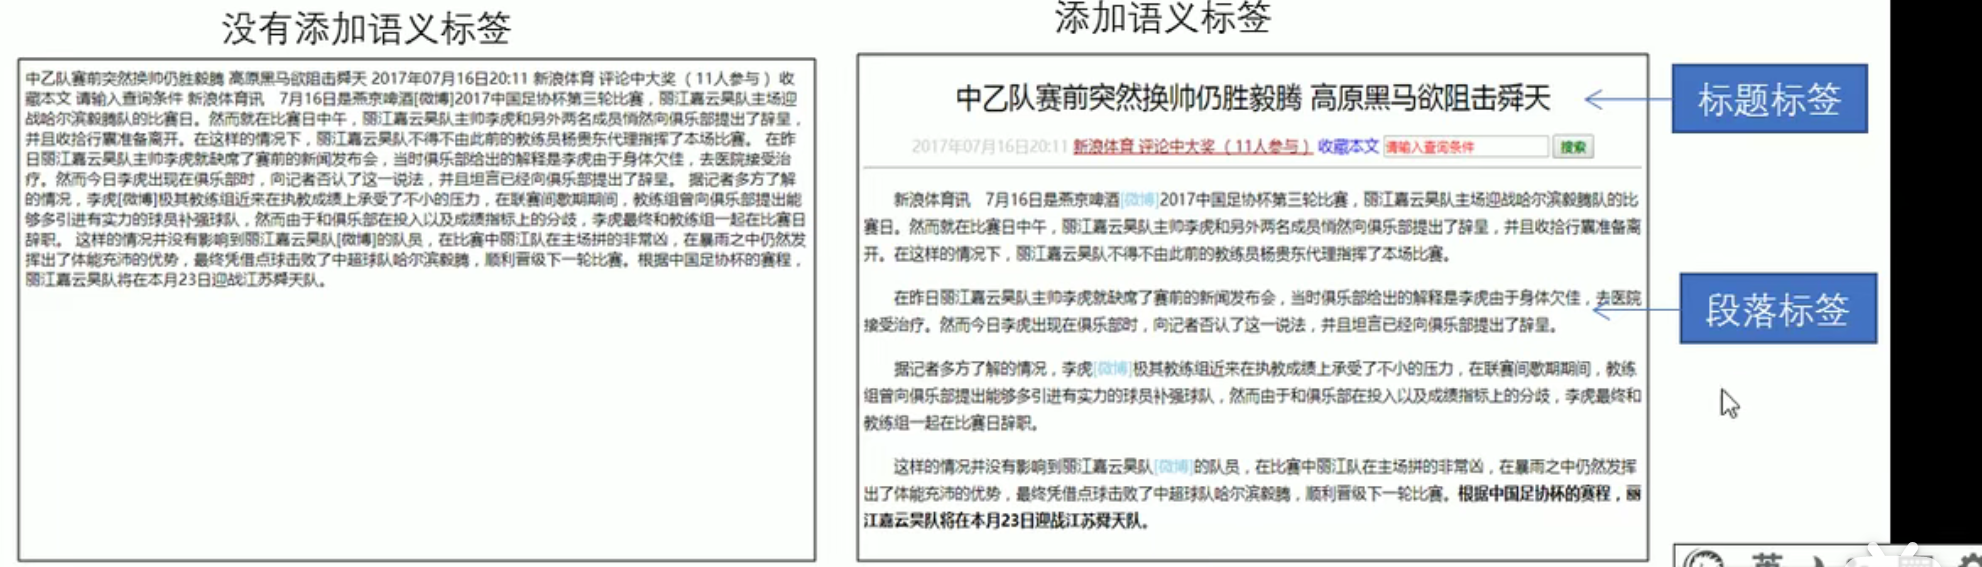
\includegraphics{fig/1-6} 

}

\caption{语义标签}\label{fig:unnamed-chunk-1}
\end{figure}

\hypertarget{ux6807ux9898ux6807ux7b7e}{%
\section{标题标签}\label{ux6807ux9898ux6807ux7b7e}}

为了使网页更具有语义化,我们经常会在页面中用到标题标签。HTML提供了6个等级的网页标题,即\texttt{\textless{}h1\textgreater{}} - \texttt{\textless{}h6\textgreater{}}。

\begin{Shaded}
\begin{Highlighting}[]
\KeywordTok{\textless{}h1\textgreater{}}\NormalTok{我是一级标题}\KeywordTok{\textless{}/h1\textgreater{}}
\end{Highlighting}
\end{Shaded}

h单词head 的缩写,意为头部、标题。
\textbf{标签语义}:作为标题使用,并且依据重要性递减。\\
特点:

\begin{itemize}
\tightlist
\item
  加了标题的文字会变的加粗,字号也会依次变大。
\item
  一个标题独占一行。
\end{itemize}

\begin{Shaded}
\begin{Highlighting}[]
\KeywordTok{\textless{}h1\textgreater{}}\NormalTok{标题一共六级选,}\KeywordTok{\textless{}/h1\textgreater{}}
\KeywordTok{\textless{}h2\textgreater{}}\NormalTok{文字加粗一行显。}\KeywordTok{\textless{}/h2\textgreater{}}
\KeywordTok{\textless{}h3\textgreater{}}\NormalTok{由大到小依次减,}\KeywordTok{\textless{}/h3\textgreater{}}
\KeywordTok{\textless{}h4\textgreater{}}\NormalTok{从重到轻随之变。}\KeywordTok{\textless{}/h4\textgreater{}}
\KeywordTok{\textless{}h5\textgreater{}}\NormalTok{语法规范书写后,}\KeywordTok{\textless{}/h5\textgreater{}}
\KeywordTok{\textless{}h6\textgreater{}}\NormalTok{具体效果刷新见。}\KeywordTok{\textless{}/h6\textgreater{}}
\end{Highlighting}
\end{Shaded}

\hypertarget{ux6bb5ux843dux6807ux7b7e}{%
\section{段落标签}\label{ux6bb5ux843dux6807ux7b7e}}

在网页中,要把文字有条理地显示出来,就需要将这些文字分段显示。在HTML标签中,\texttt{\textless{}p\textgreater{}}标签用于定义段落,它可以将整个网页分为若干个段落。

\begin{Shaded}
\begin{Highlighting}[]
\KeywordTok{\textless{}p\textgreater{}}\NormalTok{我是一个段落标签}\KeywordTok{\textless{}/p\textgreater{}}
\end{Highlighting}
\end{Shaded}

p是单词paragraph的缩写,意为段落。\textbf{标签语义}:可以把HTML文档分割为若干段落。

特点∶

\begin{itemize}
\tightlist
\item
  文本在一个段落中会根据浏览器窗口的大小自动换行。
\item
  段落和段落之间保有空隙。
\end{itemize}

\hypertarget{ux6362ux884cux6807ux7b7e}{%
\section{换行标签}\label{ux6362ux884cux6807ux7b7e}}

在HTML中,一个段落中的文字会从左到右依次排列,直到浏览器窗口的右端,然后才自动换行。如果希望某段文本强制换行显示,就需要使用换行标签\texttt{\textless{}br\ /\textgreater{}}。

\begin{Shaded}
\begin{Highlighting}[]
\KeywordTok{\textless{}br} \KeywordTok{/\textgreater{}}
\end{Highlighting}
\end{Shaded}

br是单词break的缩写,意为打断、换行。标签语义∶强制换行。

特点︰

\begin{itemize}
\tightlist
\item
  \texttt{\textless{}br\ /\textgreater{}}是个单标签。
\item
  \texttt{\textless{}br\ /\textgreater{}}标签只是简单地开始新的一行,跟段落不一样,段落之间会插入一些垂直的间距。
\end{itemize}

\hypertarget{ux6587ux672cux683cux5f0fux5316ux6807ux7b7e}{%
\section{文本格式化标签}\label{ux6587ux672cux683cux5f0fux5316ux6807ux7b7e}}

在网页中,有时需要为文字设置粗体、斜体或下划线等效果,这时就需要用到HTML中的文本格式化标签,使文字以特殊的方式显示。
标签语义:突出重要性,比普通文字更重要.

\begin{table}

\caption{\label{tab:unnamed-chunk-6}文本格式化标签}
\centering
\begin{tabular}[t]{lllll}
\toprule
语义 & 标签 & 单词 & 实例 & 说明\\
\midrule
加粗 & `<strong></strong>`或者`<b></b>` & strong & <strong>加粗</strong> & 更推荐使用`<strong>`标签加粗语义更强烈\\
倾斜 & `<em></em>`或者`<i></i>` & emphasize & <em>斜体</em> & 更推荐使用`<em>`标签加粗语义更强烈\\
删除线 & `<del></del>`或者`<s></s>` & delete & <del>删除线</del> & 更推荐使用`<del>`标签加粗语义更强烈\\
下划线 & `<ins></ins>`或者`<u></u>` & inserted & <ins>下划线</ins> & 更推荐使用`<ins>`标签加粗语义更强烈\\
\bottomrule
\end{tabular}
\end{table}

\hypertarget{ux5e03ux5c40ux6807ux7b7e}{%
\section{布局标签}\label{ux5e03ux5c40ux6807ux7b7e}}

\texttt{\textless{}div\textgreater{}}和\texttt{\textless{}span\textgreater{}}是没有语义的,它们就是一个盒子,用来装内容的。

\begin{Shaded}
\begin{Highlighting}[]
\KeywordTok{\textless{}div\textgreater{}}\NormalTok{这是头部}\KeywordTok{\textless{}/div\textgreater{}}
\KeywordTok{\textless{}span\textgreater{}}\NormalTok{今日价格}\ErrorTok{\textless{}}\NormalTok{/ span\textgreater{}}
\end{Highlighting}
\end{Shaded}

div是division的缩写,表示分割、分区。span意为跨度、跨距。

特点∶

\begin{itemize}
\tightlist
\item
  \texttt{\textless{}div\textgreater{}}标签用来布局,但是现在一行只能放一个

  。大盒子
\item
  \texttt{\textless{}span\textgreater{}}标签用来布局,一行上可以多个。小盒子
\end{itemize}

\hypertarget{ux56feux50cfux6807ux7b7eux548cux8defux5f84}{%
\section{图像标签和路径}\label{ux56feux50cfux6807ux7b7eux548cux8defux5f84}}

\hypertarget{ux56feux50cfux6807ux7b7e}{%
\subsection{图像标签}\label{ux56feux50cfux6807ux7b7e}}

在HTML标签中,\texttt{\textless{}img\textgreater{}}标签用于定义HTML页面中的图像。

\begin{Shaded}
\begin{Highlighting}[]
\KeywordTok{\textless{}img}\OtherTok{ src=}\StringTok{"图像URL”/\textgreater{}}
\end{Highlighting}
\end{Shaded}

img单词image的缩写,意为图像。
src是标签的必须属性,是单词source的缩写。它用于指定图像文件的路径和文件名。

所谓属性︰简单理解就是属于这个图像标签的特性。

\begin{table}

\caption{\label{tab:unnamed-chunk-9}图像标签常见属性}
\centering
\begin{tabular}[t]{llll}
\toprule
属性 & 属性值 & 单词 & 说明\\
\midrule
src & 图片路径 & source & 必须属性\\
alt & 文本 & alternate & 替换文本,图像不能显示的文字\\
title & 文本 & title & 提示文本。鼠标放到图像上,显示的文字\\
width & 像素 & width & 设置图像的宽度\\
heigth & 像素 & heigth & 设置图像的高度\\
\addlinespace
border & 像素 & border & 设置图像的边框粗细\\
\bottomrule
\end{tabular}
\end{table}

图像标签属性注意点∶

\begin{itemize}
\tightlist
\item
  图像标签可以拥有多个属性,必须写在标签名的后面。
\item
  属性之间不分先后顺序,标签名与属性、属性与属性之间均以空格分
\item
  属性采取键值对的格式,即key= ``value''的格式,属性=``属性值''
\end{itemize}

重点掌握点:

\begin{itemize}
\tightlist
\item
  请说出图像标签哪个属性是必须要写的?
\item
  请说出图像标签中alt和title属性区别?
\end{itemize}

\hypertarget{ux8defux5f84}{%
\subsection{路径}\label{ux8defux5f84}}

实际工作中,我们的文件不能随便乱放,否则用起来很难快速的找到他们,因此我们需要一个文件夹来管理他们。

\textbf{目录文件夹}:就是普通文件夹,里面只不过存放了我们做页面所需要的相关素材,比如html文件、图片等。

\textbf{根目录}:打开目录文件夹的第一层就是根目录.

VSCode打开目录文件夹:文件→打开文件→选择目录文件夹,后期方便管理文件

页面中的图片会非常多,通常我们会新建一个文件夹来存放这些图像文件( images ),这时再查找图像,就需要采用``路径''的方式来指定图像文件的位置。

路径可以分为︰

\begin{itemize}
\tightlist
\item
  相对路径
\item
  绝对路径
\end{itemize}

\textbf{相对路径}:以引用文件所在位置为参考基础,而建立出的目录路径。这里简单来说,图片相对于HTML页面的位置。

\begin{table}

\caption{\label{tab:unnamed-chunk-10}相对路径}
\centering
\begin{tabular}[t]{llll}
\toprule
相对路径分类 & 符号 & 说明 & 例子\\
\midrule
同一级路径 &  & 图像文件位于HTML文件同一级 & `<img src="baidu.gif" />`\\
下一级路劲 & / & 图像文件位于HTML文件下一级 & `<img src="images/baidu.gif" />`\\
上一级路径 & ../ & 图像文件位于HTML文件上一级如 & `<img src="../baidu.gif" />`\\
\bottomrule
\end{tabular}
\end{table}

以此类推,上上一级路径就是 \texttt{\textless{}img\ src="../../baidu.gif"\ /\textgreater{}}

相对路径是从代码所在的这个文件出发,去寻找目标文件的,而我们这里所说的上一级、下一级和同一级就是图片相对于HTML页面的位置。

\textbf{绝对路径}︰是指目录下的绝对位置,直接到达目标位置,通常是从盘符开始的路径。
例如,\texttt{“D:\textbackslash{}web\textbackslash{}imglogo.gif”}或完整的网络地址\texttt{“http://www.itcast.cn/images/logo.gif”}。

\hypertarget{ux8d85ux94feux63a5}{%
\section{超链接}\label{ux8d85ux94feux63a5}}

在HTML标签中,\texttt{\textless{}a\textgreater{}}标签用于定义超链接,作用是从一个页面连接到另一个页面。

\hypertarget{ux94feux63a5ux7684ux8bedux6cd5ux683cux5f0f}{%
\subsection{链接的语法格式}\label{ux94feux63a5ux7684ux8bedux6cd5ux683cux5f0f}}

\begin{Shaded}
\begin{Highlighting}[]
\KeywordTok{\textless{}a}\OtherTok{ href=}\StringTok{"跳转目标"}\OtherTok{ target=}\StringTok{"目标窗口的弹出方式"}\KeywordTok{\textgreater{}}\NormalTok{文本或图像}\KeywordTok{\textless{}/a\textgreater{}}
\end{Highlighting}
\end{Shaded}

a是单词anchor的缩写,意为∶锚。

两个属性的作用如下:

\begin{table}

\caption{\label{tab:unnamed-chunk-12}超链接标签}
\centering
\begin{tabular}[t]{ll}
\toprule
属性 & 作用\\
\midrule
href & 用于指定链接目标的url地址,是必须属性,当为标签应用href属性时,它就具有了超链接的功能\\
target & 用于指定链接页面的打开方式,其中\_self为默认值,\_\_blank为在新窗口中打开方式。\\
\bottomrule
\end{tabular}
\end{table}

注:href是Hypertext REFerence,超文本参考的缩写

\hypertarget{ux94feux63a5ux7684ux5206ux7c7b}{%
\subsection{链接的分类}\label{ux94feux63a5ux7684ux5206ux7c7b}}

\begin{itemize}
\tightlist
\item
  外部链接:例如\texttt{\textless{}a\ href="http://www.qq.com"\ target="\_blank"\textgreater{}腾讯\textless{}/a\textgreater{}}
\item
  内部链接:例如\texttt{\textless{}a\ href="index.html"\ target="\_self"\textgreater{}首页\textless{}/a\textgreater{}}
\item
  空链接:如果当时没有确定链接目标时,如\texttt{\textless{}a\ href="\#"\textgreater{}首页\textless{}/a\ \textgreater{}}
\item
  下载链接:如果href里面地址是一个文件或者压缩包,会下载这个文件。
\item
  网页元素链接:在网页中的各种网页元素,如文本、图像、表格、音频、视频等都可以添加超链接.
\item
  锚点链接:点我们点击链接,可以快速定位到页面中的某个位置.

  \begin{itemize}
  \tightlist
  \item
    在链接文本的href属性中,设置属性值为\#名字的形式,如\texttt{\textless{}a\ href="\#two"\textgreater{}第2集\textless{}/a\textgreater{}}
  \item
    找到目标位置标签,里面添加一个id属性=刚才的名字,如:\texttt{\textless{}h3\ id="two"\textgreater{}第2集介绍\textless{}/h3\textgreater{}}
  \end{itemize}
\end{itemize}

\hypertarget{ux6ce8ux91ca}{%
\section{注释}\label{ux6ce8ux91ca}}

如果需要在HTML文档中添加一些便于阅读和理解但又不需要显示在页面中的注释文字,就需要使用注释标签。HTML中的注释以\texttt{\textless{}!-\/-}开头,以\texttt{-\/-\textgreater{}}结束。

\begin{verbatim}
<!--注释语句-->
\end{verbatim}

快捷键:Ctrl + /

一句话:注释标签里面的内容是给程序猿看的,这个代码是不执行不显示到页面中的.
添加注释是为了更好地解释代码的功能,便于相关开发人员理解和阅读代码,程序是不会执行注释内容的。

\textbf{团队约定}:注释内容前后各一个空格字符,注释位于要注释代码的上面,单独占一行

\hypertarget{ux7279ux6b8aux5b57ux7b26}{%
\section{特殊字符}\label{ux7279ux6b8aux5b57ux7b26}}

HTML页面中,一些特殊符号很难或者不方便直接使用,此时我们就可以使用下面的字符来代替。

\begin{table}

\caption{\label{tab:unnamed-chunk-13}HTML特殊字符}
\centering
\begin{tabular}[t]{lll}
\toprule
特殊字符 & 描述 & 字符的代码\\
\midrule
< & 小于号 & `\&lt;`\\
> & 大于号 & `\&gt;`\\
空格 & 空格 & `\&nbsp;`\\
\& & 和号 & `\&amp;`\\
± & 正负号 & `\&plusmn;`\\
\addlinespace
\&copy; & 版权 & `\&copy;`\\
\&reg; & 商标 & `\&reg;`\\
\bottomrule
\end{tabular}
\end{table}

注:重点掌握小于号、大于号和空格,其余可查询
HTML特殊字符对照表。

\hypertarget{ux6848ux4f8bux5b66ux4e60}{%
\section{案例学习}\label{ux6848ux4f8bux5b66ux4e60}}

\begin{figure}

{\centering 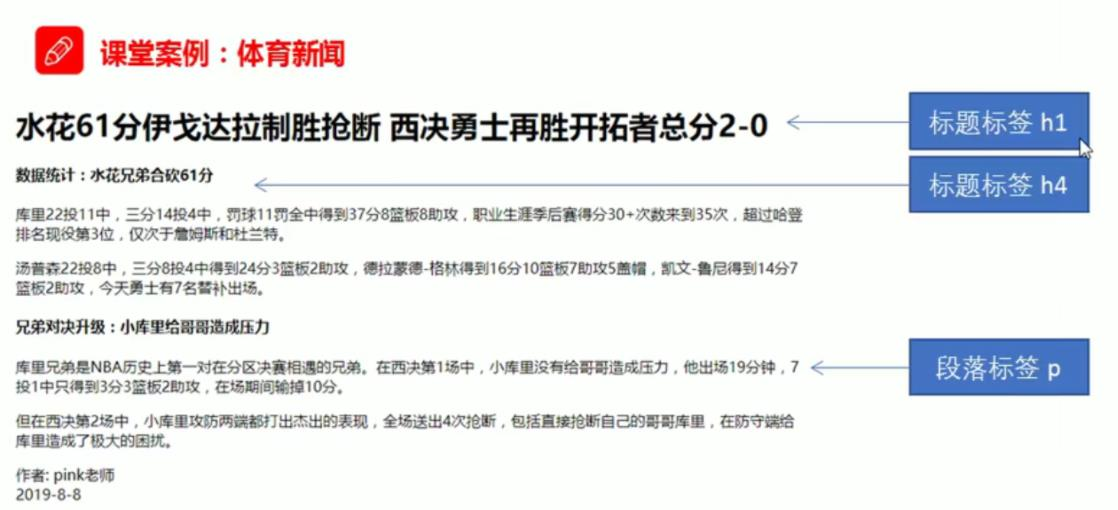
\includegraphics{fig/1-7} 

}

\caption{案例学习}\label{fig:unnamed-chunk-14}
\end{figure}

\begin{Shaded}
\begin{Highlighting}[]
\DataTypeTok{\textless{}!DOCTYPE }\NormalTok{html}\DataTypeTok{\textgreater{}}
\KeywordTok{\textless{}html}\OtherTok{ lang=}\StringTok{"en"}\KeywordTok{\textgreater{}}
\KeywordTok{\textless{}head\textgreater{}}
    \KeywordTok{\textless{}meta}\OtherTok{ charset=}\StringTok{"UTF{-}8"}\KeywordTok{\textgreater{}}
    \KeywordTok{\textless{}meta}\OtherTok{ http{-}equiv=}\StringTok{"X{-}UA{-}Compatible"}\OtherTok{ content=}\StringTok{"IE=edge"}\KeywordTok{\textgreater{}}
    \KeywordTok{\textless{}meta}\OtherTok{ name=}\StringTok{"viewport"}\OtherTok{ content=}\StringTok{"width=device{-}width, initial{-}scale=1.0"}\KeywordTok{\textgreater{}}
    \KeywordTok{\textless{}title\textgreater{}}\NormalTok{Document}\KeywordTok{\textless{}/title\textgreater{}}
\KeywordTok{\textless{}/head\textgreater{}}
\KeywordTok{\textless{}body\textgreater{}}
    \KeywordTok{\textless{}h1\textgreater{}}\NormalTok{水花61分伊戈达拉制胜抢断西决勇士再胜开拓者总分2{-}0}\KeywordTok{\textless{}/h1\textgreater{}}
    \KeywordTok{\textless{}h4\textgreater{}}\NormalTok{数据统计:水花兄弟合砍61分}\KeywordTok{\textless{}/h4\textgreater{}}
    \KeywordTok{\textless{}p\textgreater{}}
\NormalTok{        库里22投11中,三分14投4中,罚球11罚全中得到37分8篮板8助攻,职业生涯季后赛得分30+次数来到35次}
\NormalTok{        超过哈登排名现役第3位,仅次于詹姆斯和杜兰特。}
    \KeywordTok{\textless{}/p\textgreater{}}   
    \KeywordTok{\textless{}p\textgreater{}}
\NormalTok{        汤普森22投8中,三分8投4中得到24分3篮板2助攻,德拉蒙德{-}格林得到16分10篮板7助攻5盖帽,凯文{-}鲁尼得到14分7篮板2助攻,今天勇士有7名替补出场。}
    \KeywordTok{\textless{}/p\textgreater{}}
    \KeywordTok{\textless{}h4\textgreater{}}\NormalTok{兄弟对决升级:小库里给哥哥造成压力}\KeywordTok{\textless{}/h4\textgreater{}}
    \KeywordTok{\textless{}p\textgreater{}}
\NormalTok{        库里兄弟是NBA历史上第一对在分区决赛相遇的兄弟。在西决第1场中,小库里没有给哥哥造成压力,他出场19分钟,7投1中只得到3分3篮板2助攻,在场期间输掉10分。}
    \KeywordTok{\textless{}/p\textgreater{}}
    \KeywordTok{\textless{}p\textgreater{}}
\NormalTok{        但在西决第2场中,小库里攻防两端都打出杰出的表现,全场送出4次抢断,包括直接抢断自己的哥哥库里,在防守端给库里造成了极大的困扰。}
    \KeywordTok{\textless{}/p\textgreater{}}
    \KeywordTok{\textless{}p\textgreater{}}
\NormalTok{        作者: pink老师}\KeywordTok{\textless{}br} \KeywordTok{/\textgreater{}}\NormalTok{2019{-}8{-}8}
    \KeywordTok{\textless{}/p\textgreater{}}
\KeywordTok{\textless{}/body\textgreater{}}
\KeywordTok{\textless{}/html\textgreater{}}
\end{Highlighting}
\end{Shaded}

\hypertarget{part-ux9644ux5f55}{%
\part{附录}\label{part-ux9644ux5f55}}

\hypertarget{vscodeux5e38ux7528ux64cdux4f5c}{%
\chapter{Vscode常用操作}\label{vscodeux5e38ux7528ux64cdux4f5c}}

快捷键

\begin{itemize}
\tightlist
\item
  创建文件:\texttt{Ctrl+}N`
\item
  保存文件:\texttt{Ctrl+}S`
\item
  放大页面:\texttt{Ctrl}+\texttt{+}
\item
  缩小页面:\texttt{Ctrl}+\texttt{-}
\item
  预览页面:\texttt{Alt}+\texttt{B},或单击鼠标右键,在弹出窗口中点击\texttt{Open\ in\ Default\ Browser}
\item
  自动换行:\texttt{Alt}+\texttt{Z},或在\texttt{查看}中选择\texttt{自动换行}
\item
  自动注释:\texttt{ctrl}+\texttt{/}
\end{itemize}

\hypertarget{section}{%
\chapter{4}\label{section}}

\printbibliography

\end{document}
